\chapter{先行研究}
\label{chap:system}

この章ではモバイル端末における文章表示における読みやすさに関する研究論文を紹介する。次に既存のライブラリについて紹介し、
本研究の立ち位置を明確にする。

\newpage

\section{読む行為と認知に関する研究}

神戸(1994)は紙媒体での日本語の文章において、一つの注視点に停留している間に情報が収集される範囲は,
被験者によって個人差があるが,9文字から12文字の範囲であることを明らかにし、
加えて、注視点の平均的な移動距離は,3文字から5文字の間であることを示した。\cite{1}
また、中篠(1999)は日本語を読む行為において、人間の視点移動は文節単位で行われる、と述べた。\cite{2}

\subsubsection{視認性}
村田らはリアルタイムでの講演会での登壇者の音声から自動で字幕を生成する際の
視認性を向上させる研究の中で、話言葉はその意味のまとまりを考慮し改行を行うことにより、
視認性が向上することを報告している。\cite{3}

また、小林らは、村田らの話し言葉のみならず、書き言葉でも文章の折返し箇所にて文節を分断しない改行レイアウトを提案、
視線が停まる回数である停留数が減少することで、通常の改行レイアウト
より読み速度が向上することを明らかにした。 \cite{4}

\begin{figure}[H]
    \centering
    \label{fig:image6}
    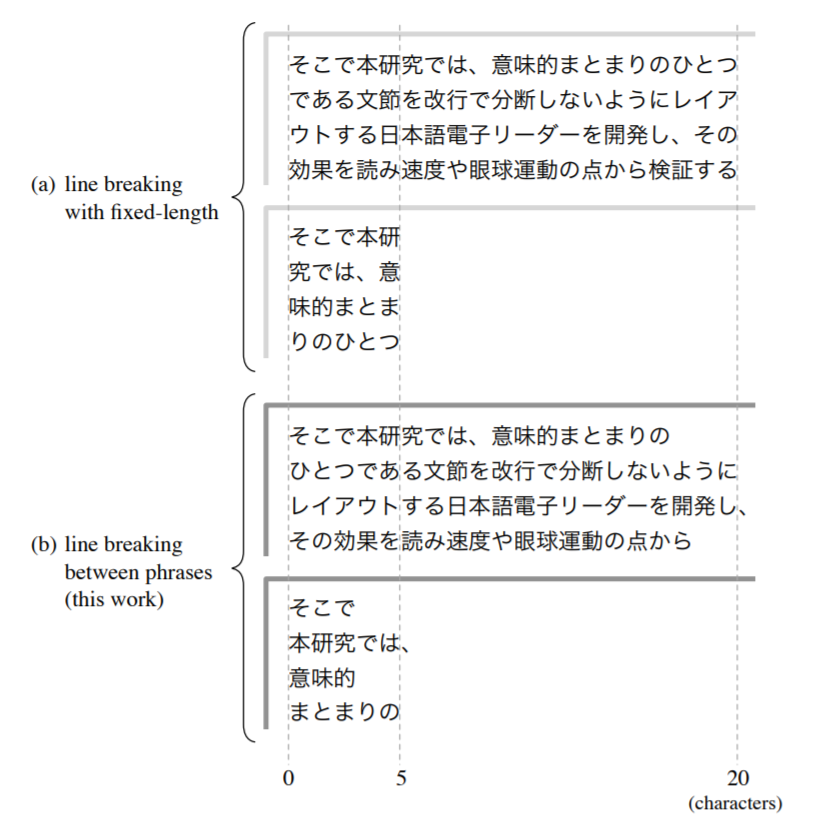
\includegraphics[width=0.6\columnwidth]{image/02/img1.png}
    \caption[文節を分断しない改行レイアウト] {文節を分断しない改行レイアウト\footnotemark[1]}
\end{figure}
\footnotetext[1]{
    引用元 文節間改行レイアウトを有する日本語リーダーの読み効率評価
}

\subsubsection{可読性}

\section{ライブラリ}
文節をもとに改行レイアウトを行う既存のライブラリとして
Budou\footnotemark[2]とmikan.js\footnotemark[3]を紹介し、その特色を述べる。

\footnotetext[2]{
    \protect\url{https://developers-jp.googleblog.com/2016/10/budou.html}
}

\footnotetext[3]{
    \protect\url{https://github.com/trkbt10/mikan.js}
}

BudouはPythonで書かれたGoogle製の形態素解析APIであるCloud Natural Language API に
を用いたライブラリであり、テンプレートエンジンのフィルタやビルドツールのタスクとして
エディタに組み込んで利用する。
単語の境界判別と構文解析を行い文節を特定し、文節ごとにdisplay:inline-blockを指定したSPANタグで囲むことで、
文章の折り返し可能な位置で改行を加えることができる。
懸念点はAPIを叩くためGoogle Cloud APIの設定や通信が必要であるがゆえにローカル環境で完結しない点と、
そのリクエストが多くなると料金が発生する点にある。また、見出し語で用いることを前提としているため、
長文で行うことが困難である。

\begin{figure}[H]
    \centering
    \label{fig:image7}
    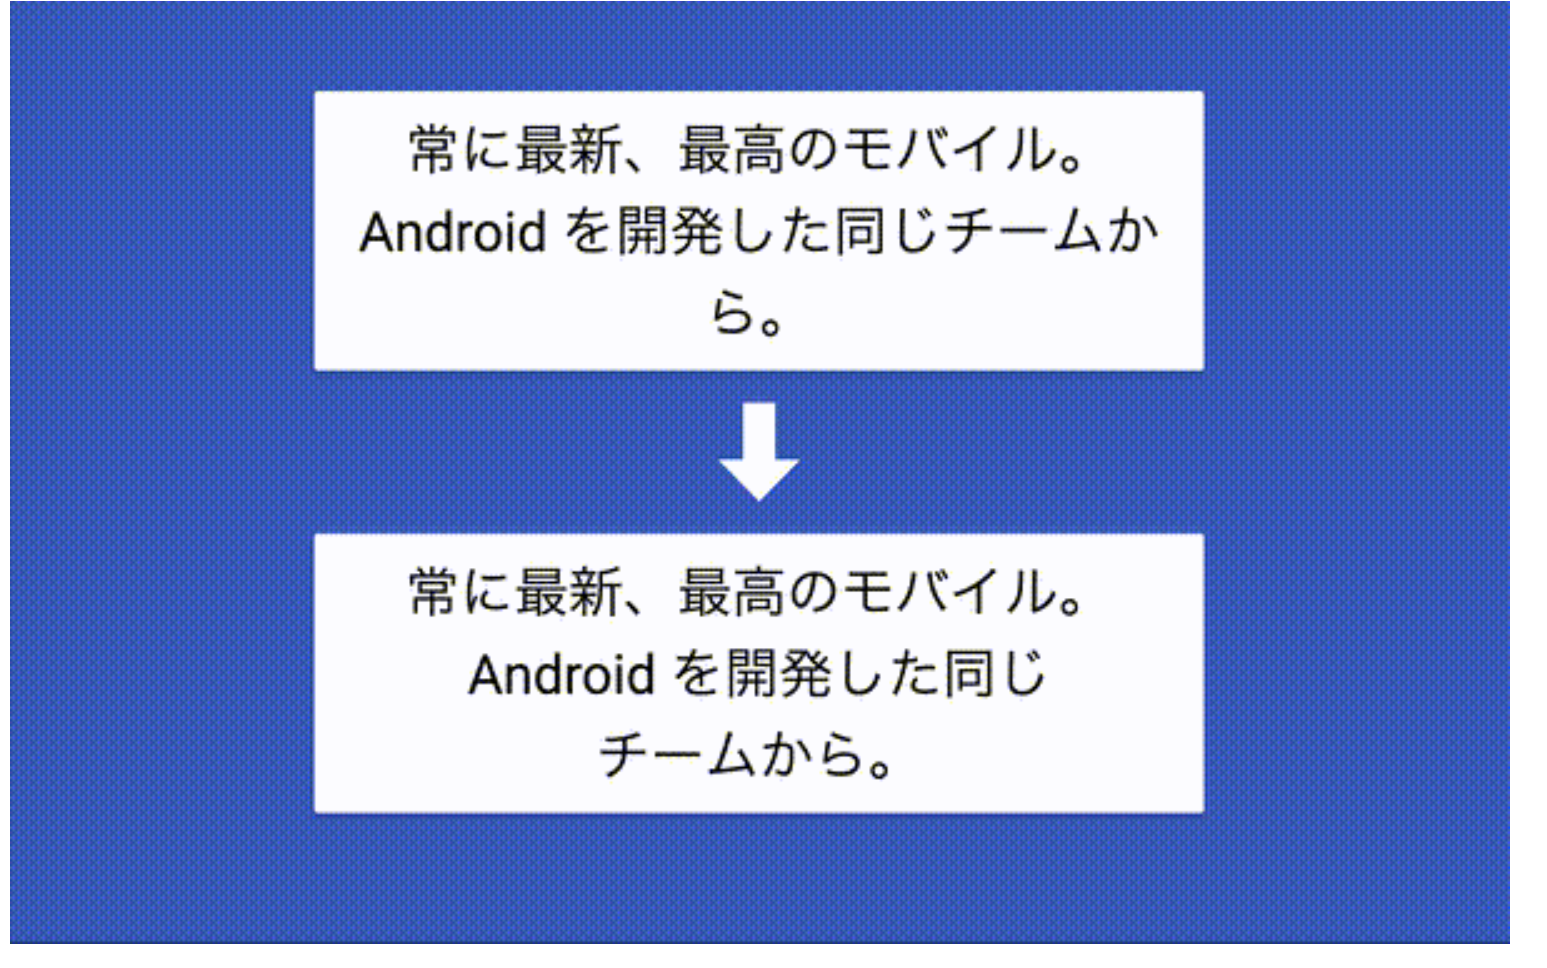
\includegraphics[width=0.6\columnwidth]{image/02/img2.png}
    \caption[Budouの動作イメージ] {Budouの動作イメージ\footnotemark[3]}
\end{figure}

mikan.jsは先述したBudouの問題点を解決するべくtrkbt10氏が開発したJavaScriptライブラリである。
簡易的な正規表現により文の区切れを特定し、Budouと同じ原理を用いて改行を加えている。
当ライブラリの利点はJavaScript製であるためにPython製のBudouよりも簡易的にフロントエンドに
組み込みやすく汎用性が高い点にあるとされる。一方の懸念点として簡易的な正規表現を利用したことにより、
大雑把な単位で文章を区切るため文章のレイアウトが損ねる点にある。またURLリンクや記号といった日本語以外の
文章に対しては精度が低いこともあげられる。また、Budouと同じ原理で改行を行うため、
同じく短文や見出し語といった限られた範囲での利用のみが想定されている。

\begin{figure}[H]
    \centering
    \label{fig:image8}
    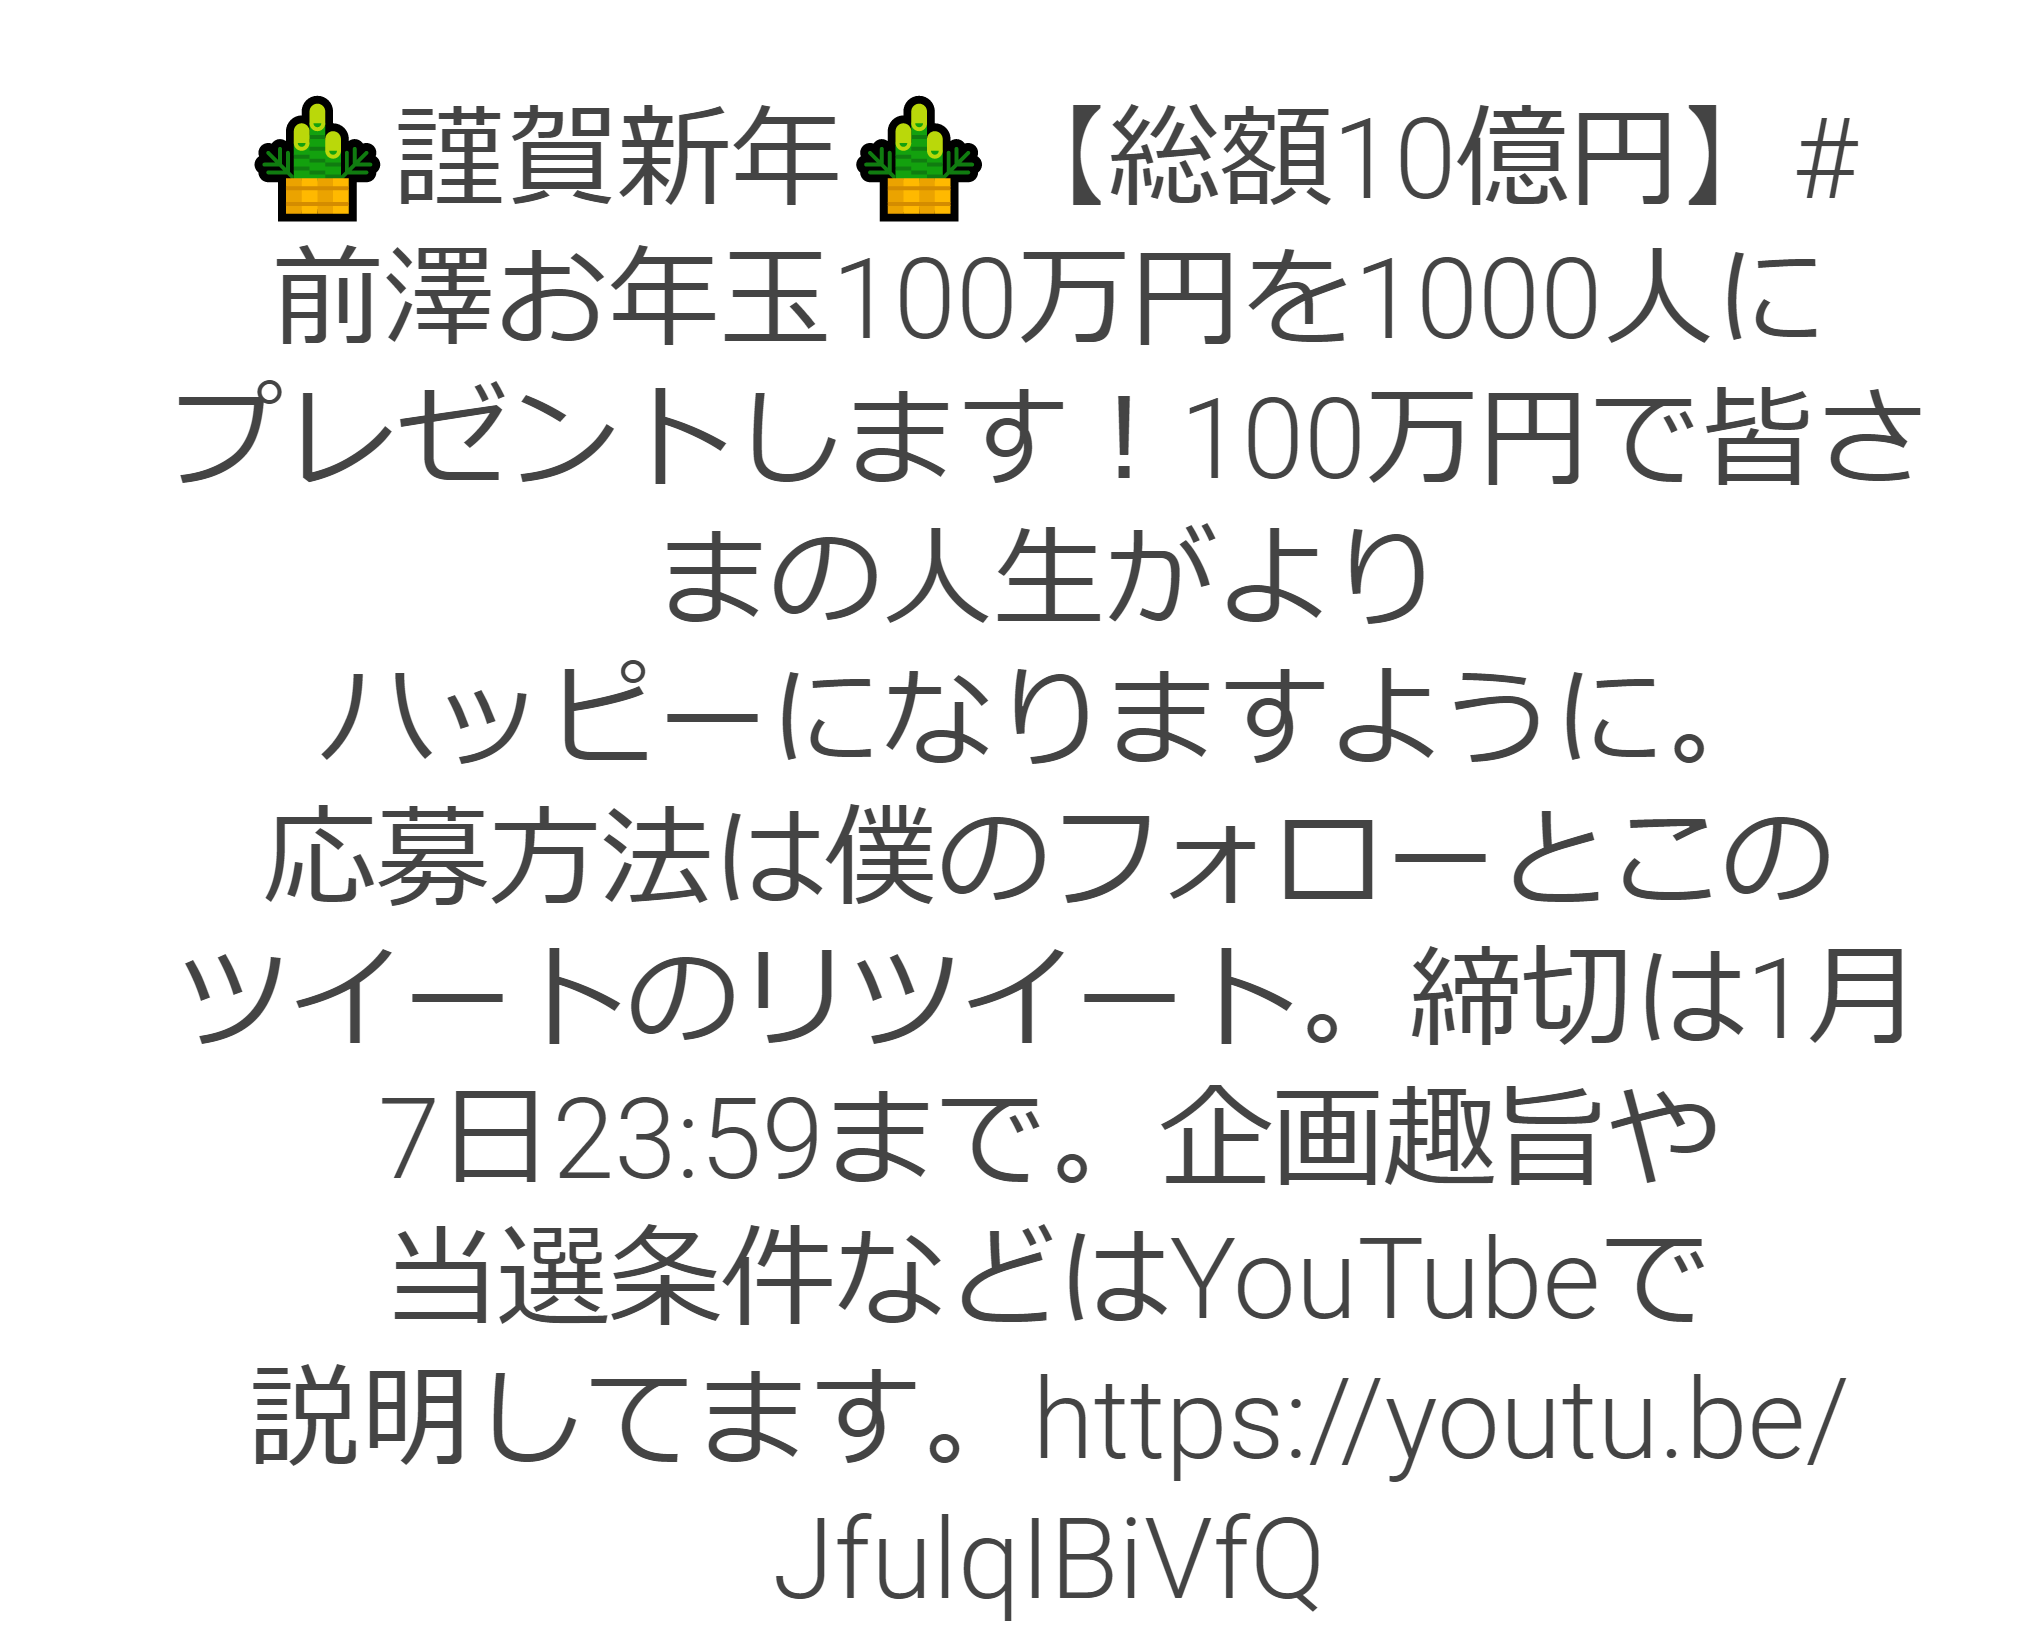
\includegraphics[width=0.6\columnwidth]{image/02/img3.png}
    \caption[mikan.jsのデモ画面にて記号やURLを表示した例] {mikan.jsのデモ画面にて記号やURLを表示した例\footnotemark[4]}
\end{figure}

\newpage

ここで双方に共通する特色として、あくまでHTMLで文章を書く際に、文章を改行位置を自動的に選定するために用いる
ライブラリであることが挙げられる。つまりは人がSNSやブログのエディタ画面では用いられることは想定していない。

\subsection{Web上の文章の特色}
本節ではWeb上の文章の特色について、先述したように現代ではブログ、
SNSでは多様なユニコードによって紙媒体では不可能である記法について述べる。

\subsubsection{DOM}
ウェブブラウザ上で文章がが表示されるのはDOM上で行われる。
「一行の長さ」といった文章がどのようにレンダリング環境は
そのDOM、およびDOMにかけられているCSSの設定によって決まる。

\subsubsection{横書き}
外国基準でウェブブラウザはデザインは発展してきたのでPC上の
文章では横書きが主流である

\subsubsection{URLリンク}
文章内にURLリンクを貼り付けてよい。クリックした場合にはそのURLへと移動する。
近年ではInstagramのハッシュタグのようなものでもURLリンクを挿入されるケースがある。

\subsubsection{句点代わりの改行}
%おまえのせいで文章のレンダリングがずれる
日本語組版に基づく方法以外に文章の文意を切り分ける方法として、改行を多用するパターンが近年では増えている。
これはDOM内を左詰めに表示される文章において余白を用いる意識したものである。
また、DOMの横幅が大きくとられている故に一行あたりが長くなることで
視認性を損ねてしまうケースを見越し、書き手側が文章の途中で改行を入れる
ケースがある。前章の研究動機にて述べた書き手と読み手側のレイアウトのズレは、
特に「句点代わりの改行」によって発生するケースが散見される。

前者はSNS等にてよく見られる記法であり、箇条書き的な記法である。
後者は視認性に関するデザインを意識していないサービスにて利用される頻度が多い。



\section{まとめ}
まず、文章のリーダビリティの研究には視認性と可読性の二種類に大別され、
文章のレイアウトの改稿は前者の分野に属することを述べた。

そして本研究では文章のレイアウトを変更する、という視認性の操作を行い
可読性には依存しないものをとして取り扱う、とした。

次に小林ら文章の視認性をあげる方法として、文節間の区切りを改行箇所として
選択し表示する研究を紹介し、その有意性を述べた。
また、MikanJSやBudouのように文節ごとにSPANタグを入れ込むことで、
PCの画面のサイズに対してレスポンシブに文節間の間が可能になるライブラリを紹介した。
これらにより文節で区切ることが可能になりつつある。

一方で、このような校正は書き手側が文章を書いているタイミングで設定する必要がある。
つまりは書き手側のためのライブラリであり、すでに書き終え、送信した文章に対して、
つまりは読み手側の環境に対してレイアウトを変更するツールするライブラリ、
サービスは散見されなかった。


